\chapter{Evaluation of performance}
\label{sec:evaluation}

To evaluate performance, benchmarks were carried out using the \mintinline{ocaml}|TimeUtil.measure_time| utility. Benchmarks were carried out on Google Chrome 99 on Debian 11 on an Intel i3-2100 CPU. The times shown are a mean of three trials. Evaluation step counts are tracked in \mintinline{ocaml}|EvalState.t| and count the number of calls to \mintinline{ocaml}|Evaluator.evaluate| as described in \Cref{sec:step-counting}.

There are a number of factors that may affect the consistency of the elapsed time benchmarks. Such factors include the quality of JSOO-generated Javascript, specifics of the Chrome V8 Javascript engine, and millisecond precision of the timing function.

Evaluation of performance of the environment model of evaluation and of the memoized hole tracking are performed on the \texttt{dev} branch and the \texttt{eval-environment} branches of the Hazel repository. The latter branch implements our changes.

The demonstration of FAR is performed on the \texttt{fill-and-resume-backend} branch. This branch is based on the \texttt{eval-environment} branch, and implements a one-step FAR operation. This branch does not achieve parity with the theoretical model of FAR presented in this work; unfinished work and future improvements to the current implementation of FAR are described in \Cref{sec:far-improvements}.

\section{Evaluation of performance using the environment model}
\label{sec:evaluation-evalenv}

To evaluate the performance of evaluation using the environment model, we benchmark the performance of a computationally-expensive function, the tree-recursive Fibonacci function. This function is chosen because it is computationally expensive and does not have a deep recursion depth\footnote{This is because Hazel does not implement tail-call optimization (TCO), and thus would overflow the stack with too much tail-recursion.}. It is also a complete program, i.e., it does not have holes and the hole renumbering and postprocessing steps are not of concern here.

For this experiment, the builtin variables and functions are removed. Restoring the builtins would be very similar to the second program variation described in \Cref{sec:eval-fib-variations}.

\subsection{A computationally expensive fibonacci program}
\label{sec:eval-fib}

The quantitative results of this experiment are shown in \Cref{tab:perf-fib-all}. The results of evaluating \Cref{fig:perf-fib} for various values of $n$ on the \texttt{dev} and \texttt{eval-environment} (abbreviated \texttt{e-e}) branches are shown in \Cref{fig:perf-fib-graph}. The \texttt{eval-environment} decreases evaluation time by a small, roughly-constant factor for all values of $n$.

\subsection{Variations on the fibonacci program}
\label{sec:eval-fib-variations}

We try out a few variations of the $\text{fib}(n)$ function, shown in \Cref{fig:perf-fib}. Results are collected for $n\in\{22,23,24,25,26\}$\footnote{These numbers were chosen somewhat arbitrarily. They are large enough to allow for reproducible results, and small enough to prevent excessively long runtimes.}. The first variation is shown in \Cref{fig:perf-fib-more-bindings}, which involves more global variables. The second variation is shown in \Cref{fig:perf-fib-more-branches}, in which an additional branch is added. This branch is never taken (as the third rule's pattern will always match), and it involves some instances of the variable $f$.

However, the two variations show the difference between evaluation with environments and evaluation with substitution. If we introduce additional global variables as in the first variation, we observe the behavior in \Cref{fig:perf-fib-more-vars-graph}. The performance of the evaluation with substitution is virtually unchanged, while the performance of evaluation with environments increases. We observe that the increase in evaluation time is not linear. We expect the slowdown to be logarithmic with respect to the number of elements in the environment. On the other hand, if more variables are introduced in an unevaluated branch as in the second variation, then we observe the reversal of the effects on the branches. This is shown in \Cref{fig:perf-fib-more-branches-graph}. The evaluation time when using substitution increases linearly with respect to the number of extra substitutions, but evaluation time using environments is roughly unchanged.

These variations show the expected behavior of the two evaluation methods. The raw performance difference is not very large. Substitution eagerly substitutes at binding time, whereas using environments lazily substitutes at lookup time. Introducing additional global variables increases the number of variables in each environment, slowing down evaluation with environments. However, this does not slow down substitution because these variables are never encountered after being bound. On the other hand, substitution necessarily traverses unevaluated branches, whereas evaluation with environment never reaches those branches.

\begin{listing}
  \inputhminted{perf_fib}
  \caption{A computationally expensive Hazel program with no holes}
  \label{fig:perf-fib}
\end{listing}

\begin{listing}
  \inputhminted{perf_fib_more_bindings}
  \caption{Adding global bindings to the program in \Cref{fig:perf-fib}}
  \label{fig:perf-fib-more-bindings}
\end{listing}

\begin{listing}
  \inputhminted{perf_fib_more_branches}
  \caption{Adding variable substitutions to unused branches to the program in \Cref{fig:perf-fib}}
  \label{fig:perf-fib-more-branches}
\end{listing}

\begin{singlespace}
  \begin{table}
    \centering
    \begin{subtable}{\textwidth}
      \begin{tabular}{r|c|ccccc|ccccc}
        \hline
        & & \multicolumn{5}{c|}{Variables in unused branch} & \multicolumn{5}{c}{Extra global variables} \\
        n & Regular & 2 & 4 & 6 & 8 & 10 & 2 & 4 & 6 & 8 & 10 \\
        \hline\hline
        22 & 334 & 394 & 509 & 539 & 658 & 677 & 339 & 305 & 302 & 339 & 336 \\
        23 & 478 & 599 & 695 & 835 & 1116 & 1107 & 524 & 442 & 452 & 452 & 455 \\
        24 & 775 & 929 & 1214 & 1332 & 1518 & 1686 & 744 & 700 & 729 & 794 & 708 \\
        25 & 1233 & 1502 & 1874 & 2310 & 2398 & 2723 & 1171 & 1189 & 1134 & 1104 & 1231 \\
        26 & 2019 & 2391 & 2939 & 3399 & 3872 & 4417 & 1841 & 1747 & 1761 & 1773 & 1780 \\
        \hline\hline
      \end{tabular}
      \caption{\texttt{dev} branch}
      \label{tab:perf-fib-dev}
    \end{subtable} \\
    \vspace{1em}
    \begin{subtable}{\textwidth}
      \begin{tabular}{r|c|ccccc|ccccc}
        \hline
        & & \multicolumn{5}{c|}{Variables in unused branch} & \multicolumn{5}{c}{Extra global variables} \\
        n & Regular & 2 & 4 & 6 & 8 & 10 & 2 & 4 & 6 & 8 & 10 \\
        \hline\hline
        22 & 255 & 267 & 276 & 242 & 245 & 243 & 330 & 384 & 417 & 435 & 519 \\
        23 & 406 & 374 & 376 & 358 & 366 & 330 & 497 & 576 & 573 & 593 & 660 \\
        24 & 578 & 558 & 559 & 591 & 561 & 569 & 775 & 857 & 911 & 912 & 1037 \\
        25 & 851 & 883 & 871 & 864 & 888 & 908 & 1209 & 1363 & 1469 & 1473 & 1684 \\
        26 & 1318 & 1388 & 1382 & 1398 & 1399 & 1415 & 1935 & 2262 & 2302 & 2356 & 2492 \\
        \hline\hline
      \end{tabular}
      \caption{\texttt{eval-environment} branch}
      \label{tab:perf-fib-evalenv}
    \end{subtable}

    \caption{Time (ms) to compute $\text{fib}(n)$}
    \label{tab:perf-fib-all}
  \end{table}
\end{singlespace}

\begin{figure}
  \centering
  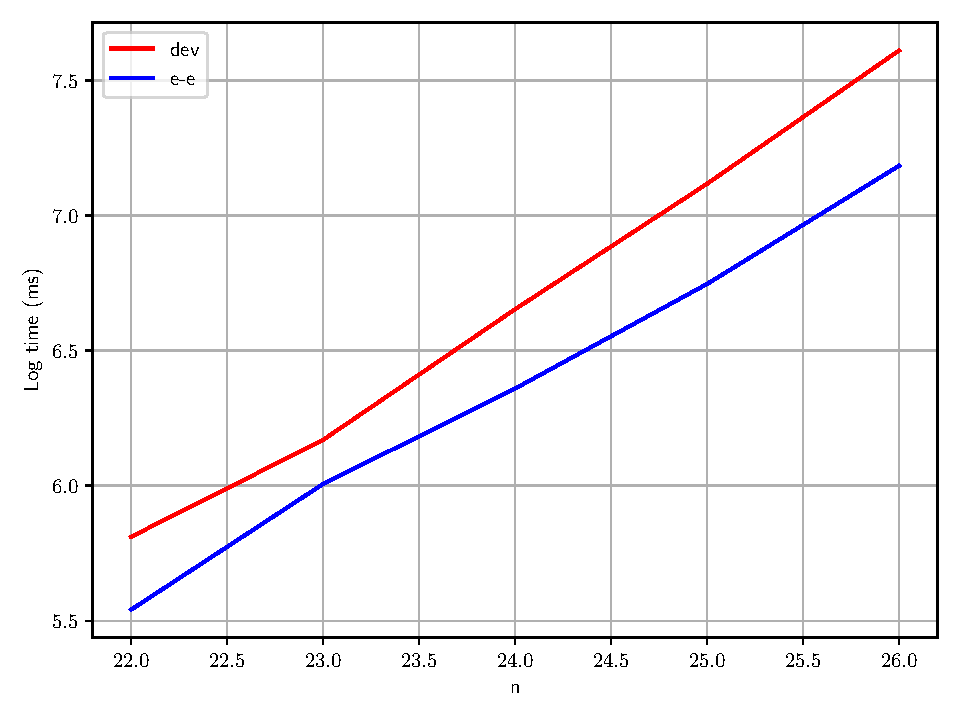
\includegraphics[width=0.7\textwidth]{img/perf_fib.pdf}
  \caption{Performance of evaluating $\text{fib}(n)$}
  \label{fig:perf-fib-graph}
\end{figure}

\begin{figure}
  \centering
  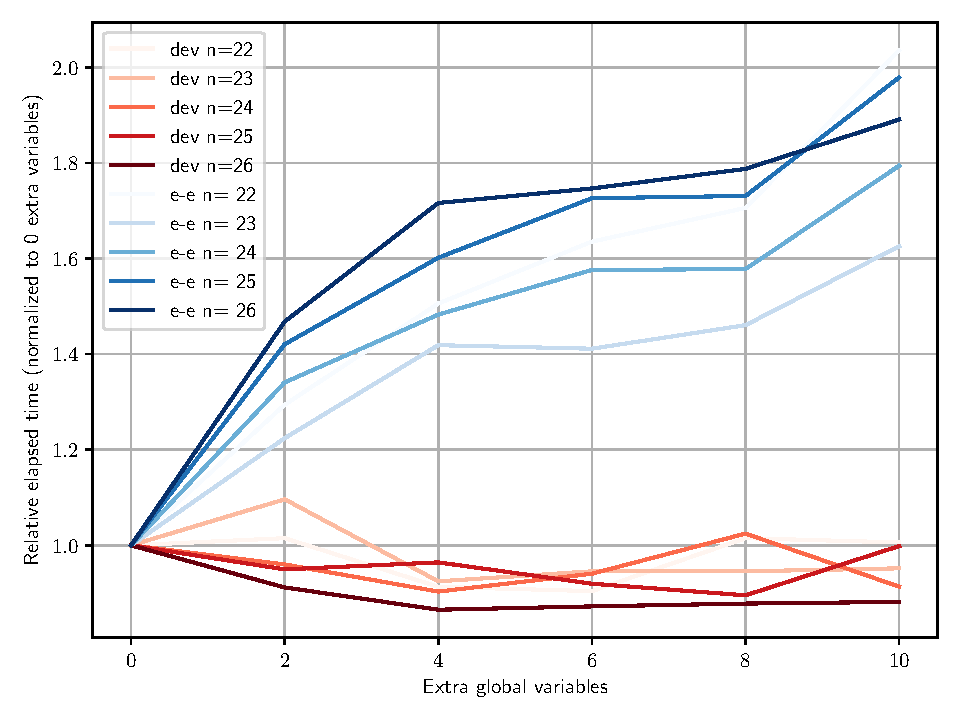
\includegraphics[width=0.7\textwidth]{img/perf_fib_more_vars.pdf}
  \caption{Performance of evaluating $\text{fib}(n)$ with extra global variables}
  \label{fig:perf-fib-more-vars-graph}
\end{figure}

\begin{figure}
  \centering
  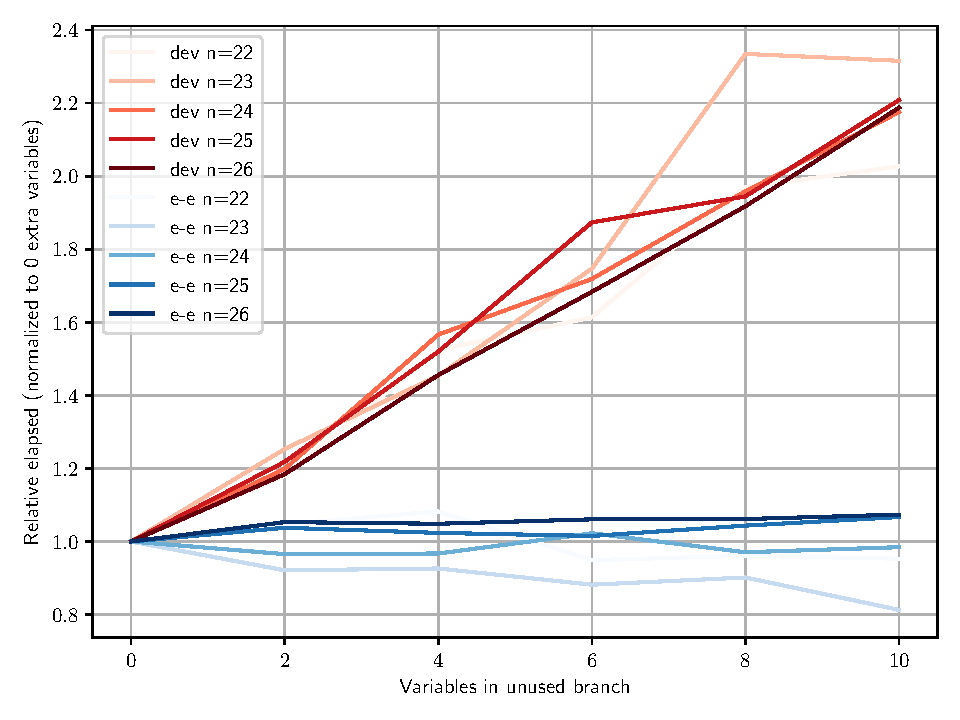
\includegraphics[width=0.7\textwidth]{img/perf_fib_more_branches.pdf}
  \caption{Performance of evaluating $\text{fib}(n)$ with an unused branch}
  \label{fig:perf-fib-more-branches-graph}
\end{figure}


\section{Postprocessing performance}
\label{sec:evaluation-renumbering}

Consider the set of programs described by \Cref{fig:hole_renumbering_problem}, which motivate the memoization of hole tracking (\Cref{sec:current-problems}) and the fast structural equality checking algorithm (\Cref{sec:fast-equals}).

We illustrate the performance issues by evaluating the performance issue. The results are shown in tabular form in \Cref{tab:perf-hole-blowup}, and visually in \Cref{fig:perf-renum-dev}. Due to the exponential blowup in elapsed time, we stop recording performance 15 \mintinline{ocaml}|let| statements.

The exponential performance blowup occurs in three places: in evaluation (due to eager substitution of holes), in hole numbering during postprocessing, and in the structural equality check in \mintinline{ocaml}|Model.update_program|. All three slowdowns occur due to the lack of memoization of hole closures when traversing a dense graph using a tree traversal algorithm.

We compare the performance to evaluation on the \texttt{eval-environment} branch which implements memoization of environments in hole numbering and structural equality. This is shown in \Cref{tab:perf-hole-blowup}, and visually in \Cref{fig:perf-renum-eev}. The evaluation time is greatly improved; total evaluation time remains negligible and never exceeds 7ms. This is the kind of evaluation time a user may expect for an ostensibly simple program.

\begin{singlespace}
  \begin{table}
    \centering
    \begin{tabular}{r|ccc|ccc}
      \hline
      & \multicolumn{3}{c|}{\texttt{dev} branch} & \multicolumn{3}{c}{\texttt{eval-environment} branch} \\
      & Evaluate & Postprocessing & Equality & Evaluate & Postprocessing & Equality \\
      \hline\hline
      1 & 0 & 0 & 0 & 0 & 1 & 0 \\
      2 & 0 & 0 & 0 & 0 & 1 & 0 \\
      3 & 1 & 2 & 0 & 0 & 1 & 0 \\
      4 & 1 & 1 & 1 & 1 & 0 & 0 \\
      5 & 1 & 1 & 2 & 0 & 3 & 0 \\
      6 & 5 & 1 & 3 & 1 & 0 & 0 \\
      7 & 4 & 5 & 6 & 2 & 2 & 0 \\
      8 & 3 & 3 & 14 & 0 & 0 & 0 \\
      9 & 6 & 18 & 33 & 1 & 0 & 1 \\
      10 & 14 & 29 & 61 & 0 & 0 & 0 \\
      11 & 13 & 41 & 91 & 3 & 2 & 0 \\
      12 & 25 & 145 & 203 & 2 & 0 & 1 \\
      13 & 65 & 578 & 383 & 2 & 0 & 0 \\
      14 & 147 & 2399 & 924 & 1 & 3 & 1 \\
      15 & 226 & 16597 & 1603 & 3 & 0 & 1 \\
      16 & & & & 1 & 0 & 1 \\
      17 & & & & 2 & 1 & 1 \\
      18 & & & & 0 & 3 & 1 \\
      19 & & & & 0 & 0 & 1 \\
      20 & & & & 3 & 4 & 0 \\
      21 & & & & 2 & 0 & 1 \\
      22 & & & & 0 & 2 & 1 \\
      23 & & & & 0 & 3 & 1 \\
      24 & & & & 0 & 6 & 1 \\
      25 & & & & 1 & 4 & 1 \\
      26 & & & & 1 & 2 & 1 \\
      \hline\hline
    \end{tabular}
    \caption{Performance of program illustrated in \Cref{fig:hole_renumbering_problem}}
    \label{tab:perf-hole-blowup}
  \end{table}
\end{singlespace}

\begin{figure}
  \centering
  \begin{subfigure}{0.7\textwidth}
    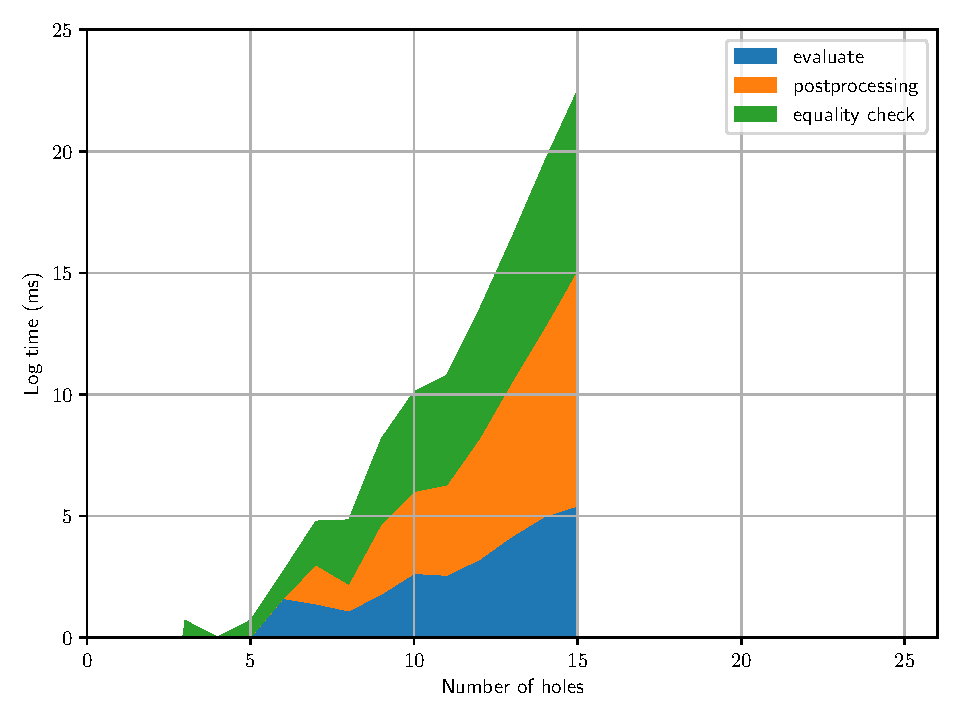
\includegraphics[width=\textwidth]{img/perf_renum_dev.pdf}
    \caption{\texttt{dev} branch}
    \label{fig:perf-renum-dev}
  \end{subfigure}
  \begin{subfigure}{0.7\textwidth}
    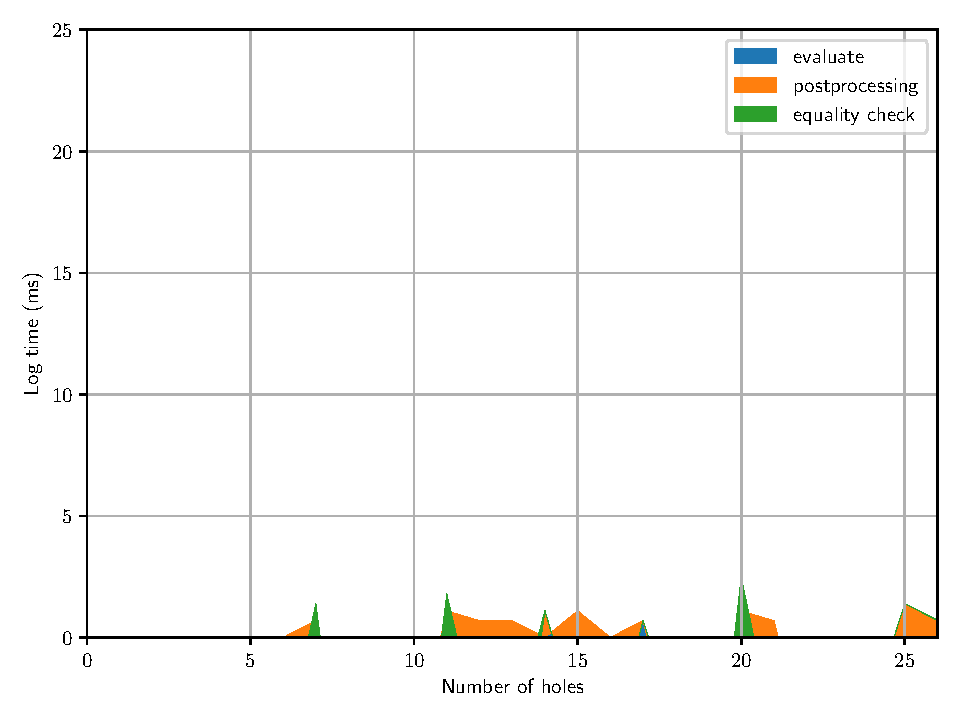
\includegraphics[width=\textwidth]{img/perf_renum_eev.pdf}
    \caption{\texttt{eval-environment} branch}
    \label{fig:perf-renum-eev}
  \end{subfigure}
  \caption{Performance of evaluating program in \Cref{fig:hole_renumbering_problem}}
  \label{fig:perf-renum}
\end{figure}

\section{FAR performance}
\label{sec:evaluation-far}

We explore two sample edit histories and the effect of FAR on the number of evaluation steps. The current implementation does not look back multiple edit states, so any fill operations will only occur if there is a valid fill from the previous edit state.

\subsection{A motivating example}
\label{sec:eval-far-motivating}

We have an example edit sequence shown in \Cref{fig:far-program-history-fib}. This shows a possible edit sequence around the motivating example in \Cref{fig:far-motivation}. In it, we have an expensive calculation, and hope to resume the result without redoing the expensive computation. The table shows the sequence of edit states (excluding movement edits). For each edit state, the number of steps is shown if regular evaluation is shown, as well as the number of steps for FAR if there is a valid fill operation. The difference in evaluation steps between the FAR evaluation and the regular evaluation is shown (Step $\Delta$), as well as the cumulative difference in evaluation steps. For operations with no valid fill operation, the step difference is zero.

We observe that for the operations before the introduction of the heavy computation $f\ 25$, there is not a significant difference in the number of steps between normal evaluation and FAR evaluation (when applicable). However, after the three steps after the introduction of this computation are valid FAR operations, and the FAR operation is extremely less expensive. A visualization for this is shown in \Cref{fig:perf-far}. With \Cref{fig:perf-no-far}, all edit states after the introduction of the heavy computation also involve the fibonacci calculation. However, in \Cref{fig:perf-far-far}, with FAR we see that subsequent calculations roughly only evaluate the filled expression. The cumulative difference in evaluation steps quickly adds up, as evidenced by \Cref{fig:far-program-history-fib}.

\subsection{Decreased performance with FAR}
\label{sec:eval-far-decreased}

Another sample program is shown in \Cref{fig:far-program-history-simple}. This explores the result of a simpler and perhaps more average program, without an expensive computation. We observe that in this case, the fill operations are typically more expensive than regular operations. This is largely due to the lack of memoization of the re-evaluation of environments in closures, which is described as future work in \Cref{sec:far-improv-memo-envs}. However, the number of evaluation steps are reasonably on the same order of magnitude as normal evaluation.

We note that we only provide evaluation step counts rather than benchmark times for this discussion of FAR. We do not find that benchmarking evaluation is necessary, as it is more or less unchanged from regular evaluation (except for treatment of closures). It may be useful to benchmark the structural diffing algorithm, but this may be more important once a multi-step FAR is implemented. The current structural diffing with a one-step FAR is a linear pass over the expression tree, which should have performance characteristics similar to other linear passes such as type-checking or elaboration, which are not a performance concern.

\begin{singlespace}
  \begin{table}
    \centering
    \begin{tabular}{p{10em}cccc}
      \hline
      Program & Steps & Steps & Step $\Delta$ & Cumulative \\
              & & (w/ FAR) & & Step $\Delta$ \\
      \hline\hline
      \inputhnfminted{far_fib_hist_1} & 7 & - & 0 & 0 \\ \hline
      \inputhnfminted{far_fib_hist_2} & 12 & 21 & 9 & 9 \\ \hline
      \inputhnfminted{far_fib_hist_3} & 17 & - & 0 & 9 \\ \hline
      \inputhnfminted{far_fib_hist_4} & 58 & 69 & 11 & 20 \\ \hline
      \inputhnfminted{far_fib_hist_5} & 4762964 & - & 0 & 20 \\ \hline
      \inputhnfminted{far_fib_hist_6} & 4762966 & 12 & -4762954 & -4762934 \\ \hline
      \inputhnfminted{far_fib_hist_7} & 4762966 & 21 & -4762954 & -9525879 \\ \hline
      \inputhnfminted{far_fib_hist_8} & 4792967 & 13 & -4792954 & -14288813 \\ \hline
      \hline
    \end{tabular}
    \caption{A program edit history with an expensive computation}
    \label{fig:far-program-history-fib}
  \end{table}
\end{singlespace}

\begin{figure}
  \centering
  \begin{subfigure}{0.7\textwidth}
    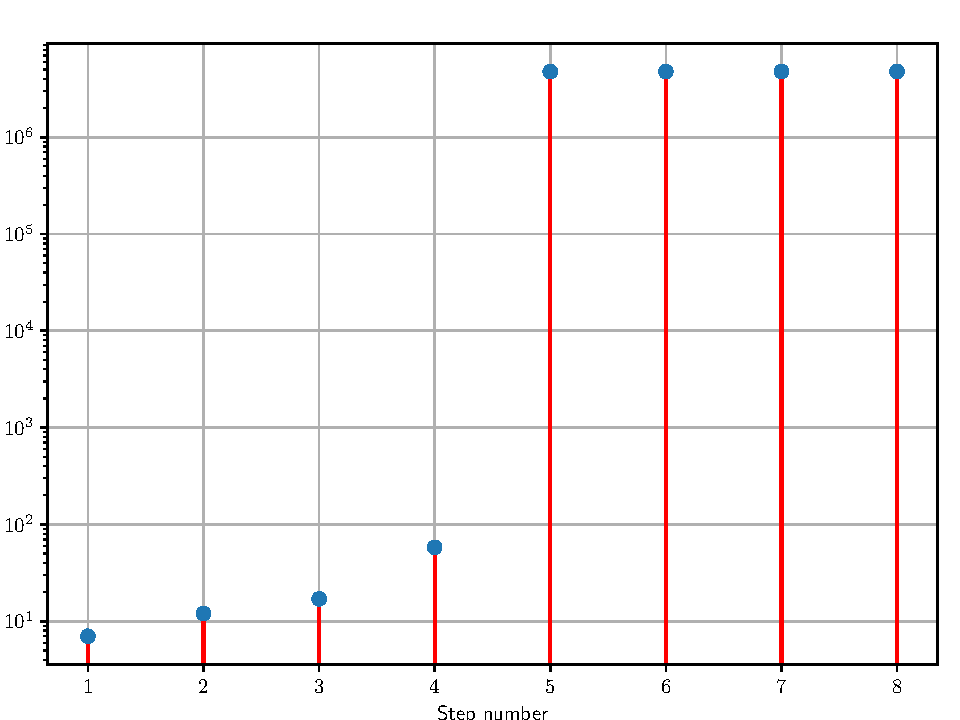
\includegraphics[width=\textwidth]{img/perf_no_far.pdf}
    \caption{Normal evaluation}
    \label{fig:perf-no-far}
  \end{subfigure}
  \begin{subfigure}{0.7\textwidth}
    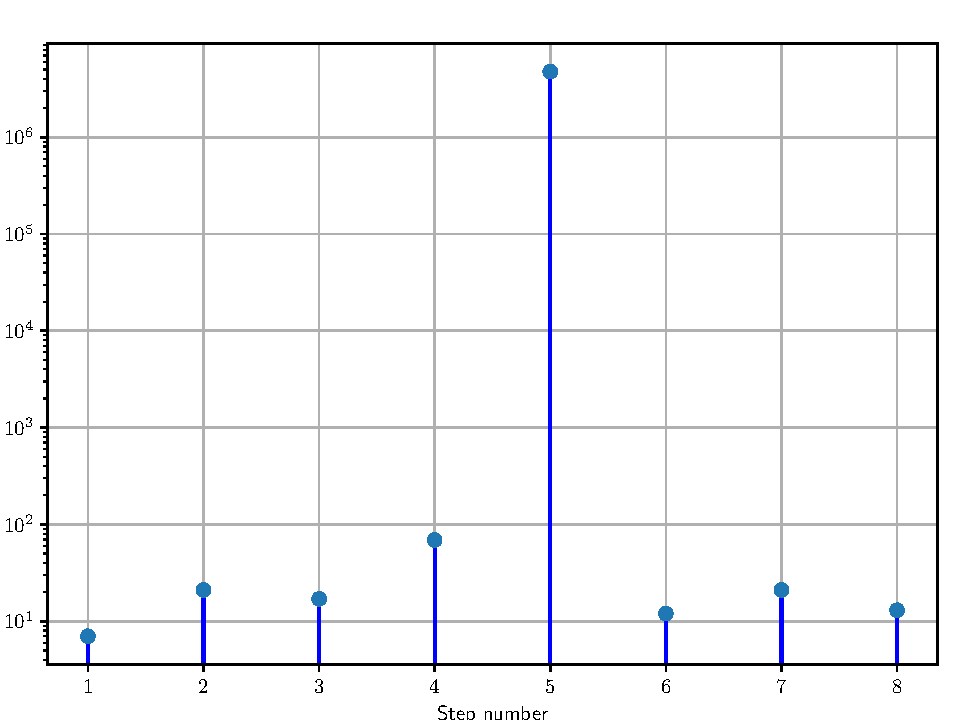
\includegraphics[width=\textwidth]{img/perf_far.pdf}
    \caption{With one-step FAR}
    \label{fig:perf-far-far}
  \end{subfigure}
  \caption{Number of evaluation steps per edit in \Cref{fig:far-program-history-fib}}
  \label{fig:perf-far}
\end{figure}

\begin{singlespace}
  \begin{table}
    \centering
    \begin{tabular}{p{10em}cccc}
      \hline
      Program & Steps & Steps & Step $\Delta$ & Cumulative \\
              & & (w/ FAR) & & Step $\Delta$ \\
      \hline\hline
      \inputhnfminted{far_hist_1} & 1 & - & 0 & 0 \\ \hline
      \inputhnfminted{far_hist_2} & 2 & 3 & 1 & 1 \\ \hline
      \inputhnfminted{far_hist_3} & 3 & - & 0 & 1 \\ \hline
      \inputhnfminted{far_hist_4} & 4 & 5 & 1 & 2 \\ \hline
      \inputhnfminted{far_hist_5} & 5 & - & 0 & 2 \\ \hline
      \inputhnfminted{far_hist_6} & 6 & 9 & 3 & 5 \\ \hline
      \inputhnfminted{far_hist_7} & 8 & 8 & 0 & 5 \\ \hline
      \inputhnfminted{far_hist_8} & 9 & 14 & 5 & 10 \\ \hline
      \inputhnfminted{far_hist_9} & 10 & 11 & 1 & 11 \\ \hline
      \inputhnfminted{far_hist_10} & 11 & 6 & -5 & 6 \\ \hline
      \hline
    \end{tabular}
    \caption{A sample edit history for a simple program}
    \label{fig:far-program-history-simple}
  \end{table}
\end{singlespace}

%%% Local Variables:
%%% mode: latex
%%% TeX-master: "main"
%%% End:
